\section{\glsfmtlong{VSL}}
\label{sec:VSL}

The \glsfirst{VSL}, commonly referred to as the RSS3 Chain, is an Ethereum Layer 2 blockchain built with OP Stack uisng Celestia as the data availability layer.
It is responsible for handling value derived from \glsfmtlong{OI} activities and applications, establishing a healthy ownership economy for the Network.

In this section, we focus on the intentions behind the \gls{VSL}'s incentive mechanism, which is designed to promote stable Node Operations to maintain the Network, and to encourage network participants to secure the Network via staking \$RSS3.
We introduce the detailed tokenomics separately in \Cref{sec:tokenomics}.

The \glsfmtlong{R3N} allocates a portion of \$RSS3 total supply to incentivize network participants, the \glsfirst{NR}, 
allocated into two reward pools: the \glsfirst{OP} and the \glsfirst{SP} for Normal Nodes, or the \glsfirst{PGP} for Public Good Nodes.
See \Cref{fig:network-rewards} and \Cref{subsec:reward_pools} for details.

\subsection{Node Operation}
\Glsfmtlong{NO}s are incentivized to operate and maintain the Network by receiving \$RSS3 as rewards.
\begin{enumerate}
    \item Anyone can become a \glsfmtlong{NO} to launch an RSS3 Node and join the RSS3 Network without requiring prior permission.
    \item A \glsfmtlong{NO} has the ability to configure Node's coverage, which directly influences the Node's capability to respond to various types of requests. A broader coverage means more computational resources are required, and a higher chance of receiving requests.
    \item A Node can be operated in either a Normal mode or a Public Good mode. A Normal Node is eligible for \glsfmtlong{NR}, but requires a deposit of \$RSS3. A Public Good Node is ineligible for \glsfmtlong{NR}, but requires no deposit.
    \item A Normal Node has a corresponding \glsentrysymbol{OP} and a \glsentrysymbol{SP}. All Public Good Nodes collectively share a single \glsentrysymbol{PGP}.
\end{enumerate}

\subsection{Node Staking}
Network participants are incentivized to stake \$RSS3 to secure the Network by receiving \$RSS3 as rewards.
\begin{enumerate}
    \item A Normal Node accepts staking into its Reward Pool, the amount of staked \$RSS3 signifies its quality. Higher quality Nodes handle more requests.
    \item A Public Good Node does not have a Reward Pool and does not participate in any form of incentivization. Staking into a \glsfmtlong{PGP} is accepted, and the stakers can assign their trust to any Public Good Node. Higher trust Nodes handle more requests.
\end{enumerate}

{
\renewcommand{\arraystretch}{1.5}
\begin{table*}[h]
    \resizebox{\textwidth}{!}{
        \begin{tabulary}{\textwidth}{|p{6cm}|p{5cm}|p{5cm}|}
            \hline
            & \textbf{Node in Normal Mode} & \textbf{Node in Public Good mode} \\ \hline
            Who can operate? & Anyone & Anyone \\ \hline
            Can \glsfmtlong{NO} specify the coverage? & Yes & Yes \\ \hline
            Is a deposit required? & Yes & No \\ \hline
            Is the deposit considered as staking, making it eligible for rewards from its own \glsentrysymbol{SP}? & No & N/A \\ \hline
            Will the Node be slashed? & Yes, its deposit and \glsentrysymbol{SP} will be slashed. A Node may be demoted to receive fewer requests. & No, but a Node may be demoted to receive fewer requests. \\ \hline
            Does the Node accept staking? & Yes. The staked tokens go to the Node’s \glsentrysymbol{SP}. RSS3-X (X being the Node’s name) Chips are issued to the stakers after staking. & No, as such a Node does not have a \glsfmtlong{SP}. Instead, stakers stake to a \glsfmtlong{PGP}. RSS3-Public Good Chips are issued to the stakers after staking. \\ \hline
            Can \glsfmtlong{NO} set an \glsfirst{Tax}? & Yes & No, a universal tax is determined by the Network. \\ \hline
            Does it have an \glsfmtlong{OP}? & Yes & No, operator rewards go to [X] \\ \hline
            Does it have a \glsfmtlong{SP}? & Yes & No, but a \glsfmtlong{PGP} with a universal incentive rate. \\ \hline
        \end{tabulary}
    }
    \caption{Comparison of two Node operation modes.}
    \label{table:node_modes}
\end{table*}
}

\subsection{Reward Pools}
\label{subsec:reward_pools}

This section introduces the three reward pools: the \glsfirst{OP}, the \glsfirst{SP}, and the \glsfirst{PGP}. See \Cref{fig:network-rewards} for an illustration.

{
\begin{figure}[tb!]
    \centering
    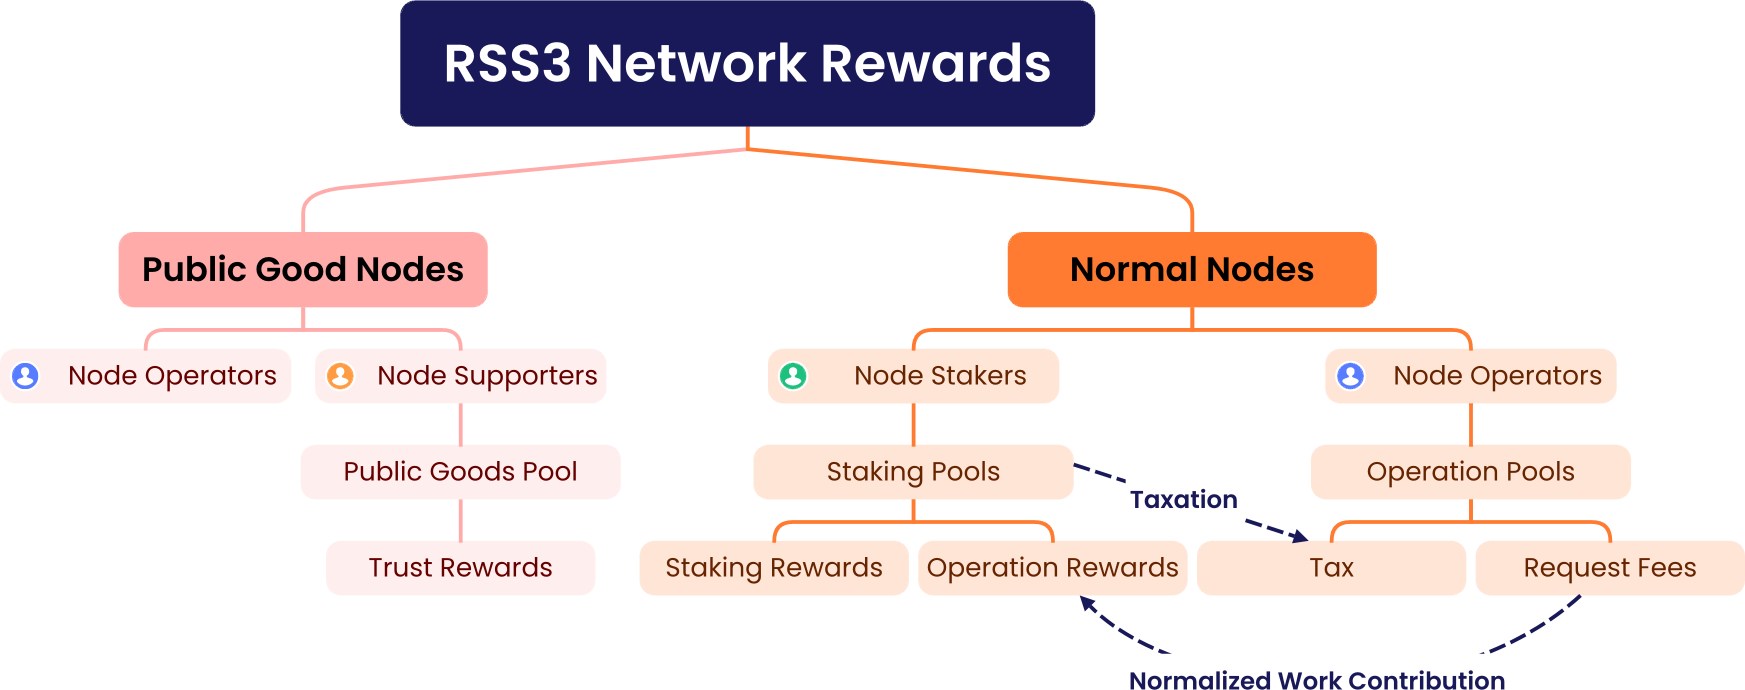
\includegraphics[width=0.9\columnwidth]{figures/network-rewards.png}
    \caption{RSS3 \glsfmtlong{NR} distribution.
    The \glsfmtlong{NR} are allocated into two reward pools: the \glsfirst{OP} and the \glsfirst{SP} for Normal Nodes, or the \glsfirst{PGP} for Public Good Nodes.
    See \Cref{subsec:reward_pools} for details.}
    \label{fig:network-rewards}
\end{figure}
}

\subsubsection{\glsfmtlong{OP} (\glsentrysymbol{OP})}
\label{subsubsec:operating_pool}

An \glsfirst{OP} is used to store tokens that are allocated to a Normal Node from three sources: 1) the \gls{Fee} collected from requests served on the \gls{DSL}, denoted \glsentrysymbol{N}; 3) the \glsfmtlong{NR} allocated based on the Node’s work; 3) the \gls{Tax} collected from the Node's \glsfirst{SP}.

The allocation of \glsfmtlong{NR} into a Node's \glsentrysymbol{OP} at the end of each epoch, is determined by the \glsfmtlong{N} (\glsentrysymbol{N}), in proportion to the total number of requests served on the \gls{DSL}.

The \glsfmtlong{NO} can set a tax rate, \glsentrysymbol{Tax}, which is applied to its \glsentrysymbol{SP}.
The tax applies to the \glsfmtlong{NR} allocated to the Node's \glsentrysymbol{SP}, not the staked tokens (REP-1: Chip Redemption Tax).

Only the corresponding \glsfmtlong{NO} can withdraw tokens from its \glsentrysymbol{OP}, and the withdrawal is subject to a waiting period imposed by the Network.

\subsubsection{\glsfmtlong{SP} (\glsentrysymbol{SP})}

A \glsfirst{SP} is used to store staked tokens for a Normal Node. Network participants can stake tokens into a Normal Node's \glsentrysymbol{SP} to increase the Node's chance to receive requests on the \gls{DSL}.

The allocation of \glsfmtlong{NR} into a Node's \glsentrysymbol{SP} at the end of each epoch, is determined by the size of the Node's \glsentrysymbol{SP}, in proportion to the total staked tokens on the \gls{VSL}.
A tax is then applied to the received Rewards, with the rate set by its \glsfmtlong{NO}.

\subsubsection{\glsfmtlong{PGP} (\glsentrysymbol{PGP})}

A \glsfirst{PGP} is a unique reward pool that is shared by all Public Good Nodes.
